%%%%%%%%%%%%%%%%%%%%%%%%%%%%%%%%%%%%%%%%%
% baposter Landscape Poster
% LaTeX Template
% Version 1.0 (11/06/13)
%
% baposter Class Created by:
% Brian Amberg (baposter@brian-amberg.de)
%
% This template has been downloaded from:
% http://www.LaTeXTemplates.com
%
% License:
% CC BY-NC-SA 3.0 (http://creativecommons.org/licenses/by-nc-sa/3.0/)
%
%%%%%%%%%%%%%%%%%%%%%%%%%%%%%%%%%%%%%%%%%

%----------------------------------------------------------------------------------------
%	PACKAGES AND OTHER DOCUMENT CONFIGURATIONS
%----------------------------------------------------------------------------------------

\documentclass[landscape,a0paper, fontscale = 0.285]{baposter} % Adjust the font scale/size here

\usepackage{graphicx} % Required for including images
\graphicspath{{figures/}} % Directory in which figures are stored

\usepackage{amsmath} % For typesetting math
\usepackage{amssymb} % Adds new symbols to be used in math mode


\usepackage{booktabs} % Top and bottom rules for tables
\usepackage{enumitem} % Used to reduce itemize/enumerate spacing
\usepackage{palatino} % Use the Palatino font
\usepackage{newpxmath}
\usepackage[font=scriptsize,labelfont=bf]{caption} % Required for specifying captions to tables and figures

\usepackage{multicol} % Required for multiple columns
\setlength{\columnsep}{1.5em} % Slightly increase the space between columns
\setlength{\columnseprule}{0mm} % No horizontal rule between columns

\usepackage{tikz} % Required for flow chart
\usetikzlibrary{shapes,arrows} % Tikz libraries required for the flow chart in the template

\newcommand{\compresslist}{ % Define a command to reduce spacing within itemize/enumerate environments, this is used right after \begin{itemize} or \begin{enumerate}
\setlength{\itemsep}{1pt}
\setlength{\parskip}{0pt}
\setlength{\parsep}{0pt}
}

\newcommand{\condensemath}{ % Define a command to reduce spacing between math
\setlength{\abovedisplayskip}{2pt}
\setlength{\belowdisplayskip}{2pt}
}


\definecolor{lightblue}{rgb}{0.671, 0.875, 1} % Defines the color used for content box headers
\definecolor{cream}{rgb}{1,0.996,0.867}
\definecolor{sky}{rgb}{0.847, 0.941, 1}
\definecolor{pastelgreen}{rgb}{0.780,1,0.549}


\begin{document}

\begin{poster}
{
headerborder=closed, % Adds a border around the header of content boxes
colspacing=1em, % Column spacing
bgColorOne=white, % Background color for the gradient on the left side of the poster
bgColorTwo=white, % Background color for the gradient on the right side of the poster
borderColor=sky, % Border color
headerColorOne=sky, % Background color for the header in the content boxes (left side)
headerColorTwo=sky, % Background color for the header in the content boxes (right side)
headerFontColor=black, % Text color for the header text in the content boxes
boxColorOne=white, % Background color of the content boxes
textborder=rounded, % Format of the border around content boxes, can be: none, bars, coils, triangles, rectangle, rounded, roundedsmall, roundedright or faded
eyecatcher=false, % Set to false for ignoring the left logo in the title and move the title left
headerheight=0.1\textheight, % Height of the header
headershape=rounded, % Specify the rounded corner in the content box headers, can be: rectangle, small-rounded, roundedright, roundedleft or rounded
headerfont=\large\sc, % Large, bold and sans serif font in the headers of content boxes
%textfont={\setlength{\parindent}{1.5em}}, % Uncomment for paragraph indentation
linewidth=2pt % Width of the border lines around content boxes
}
%----------------------------------------------------------------------------------------
%	TITLE SECTION 
%----------------------------------------------------------------------------------------
%
{\includegraphics[height=4em]{logo.png}} % First university/lab logo on the left
{\huge\bf\textsc{Economic Growth and the Agricultural Productivity Gap}\vspace{0.5em}} % Poster title
{\textsc{Nikhil Raman, B.A. Joint Honours Economics and Mathematics}} % Author names and institution
{\includegraphics[height=4em]{logo.png}} % Second university/lab logo on the right


%----------------------------------------------------------------------------------------
%	ACKNOWLEDGEMENTS
%----------------------------------------------------------------------------------------

\headerbox{Acknowledgements}{name=acknowledgements,column=0,span=2,above=bottom}{ % This block is as tall as the references block

\begin{multicols}{2}
This project would not have been possible without the support of many people. I would like to thank Professor Francisco Alvarez-Cuadrado for including me in
this project and for his guidance throughout the process, as well as 

Ph.D. candidate Shu Chen for his ideas and work. I also thank the Arts
Internship Office for selecting me for an ARIA award, and  Mr. Mark W. Gallop for funding this research. 
\end{multicols}
}

%----------------------------------------------------------------------------------------
%	INTRODUCTION
%----------------------------------------------------------------------------------------

\headerbox{Introduction}{name=objectives,column=0,span=1, row =0, above = acknowledgements}{

This project aims to understand the vast income differences across countries through the lens of
agricultural productivity. Rich countries often outperform poor countries across all
sectors of the economy; when looking at \emph{value added per worker}, a measure
of labor productivity, the top 5 countries average around 40 times higher than
the bottom 5.
However, a productivity gap is especially present in the agricultural sector
across countries,
where in \emph{real} terms, this factor is around 80 \cite{restuccia2008agriculture}.

\begin{center}
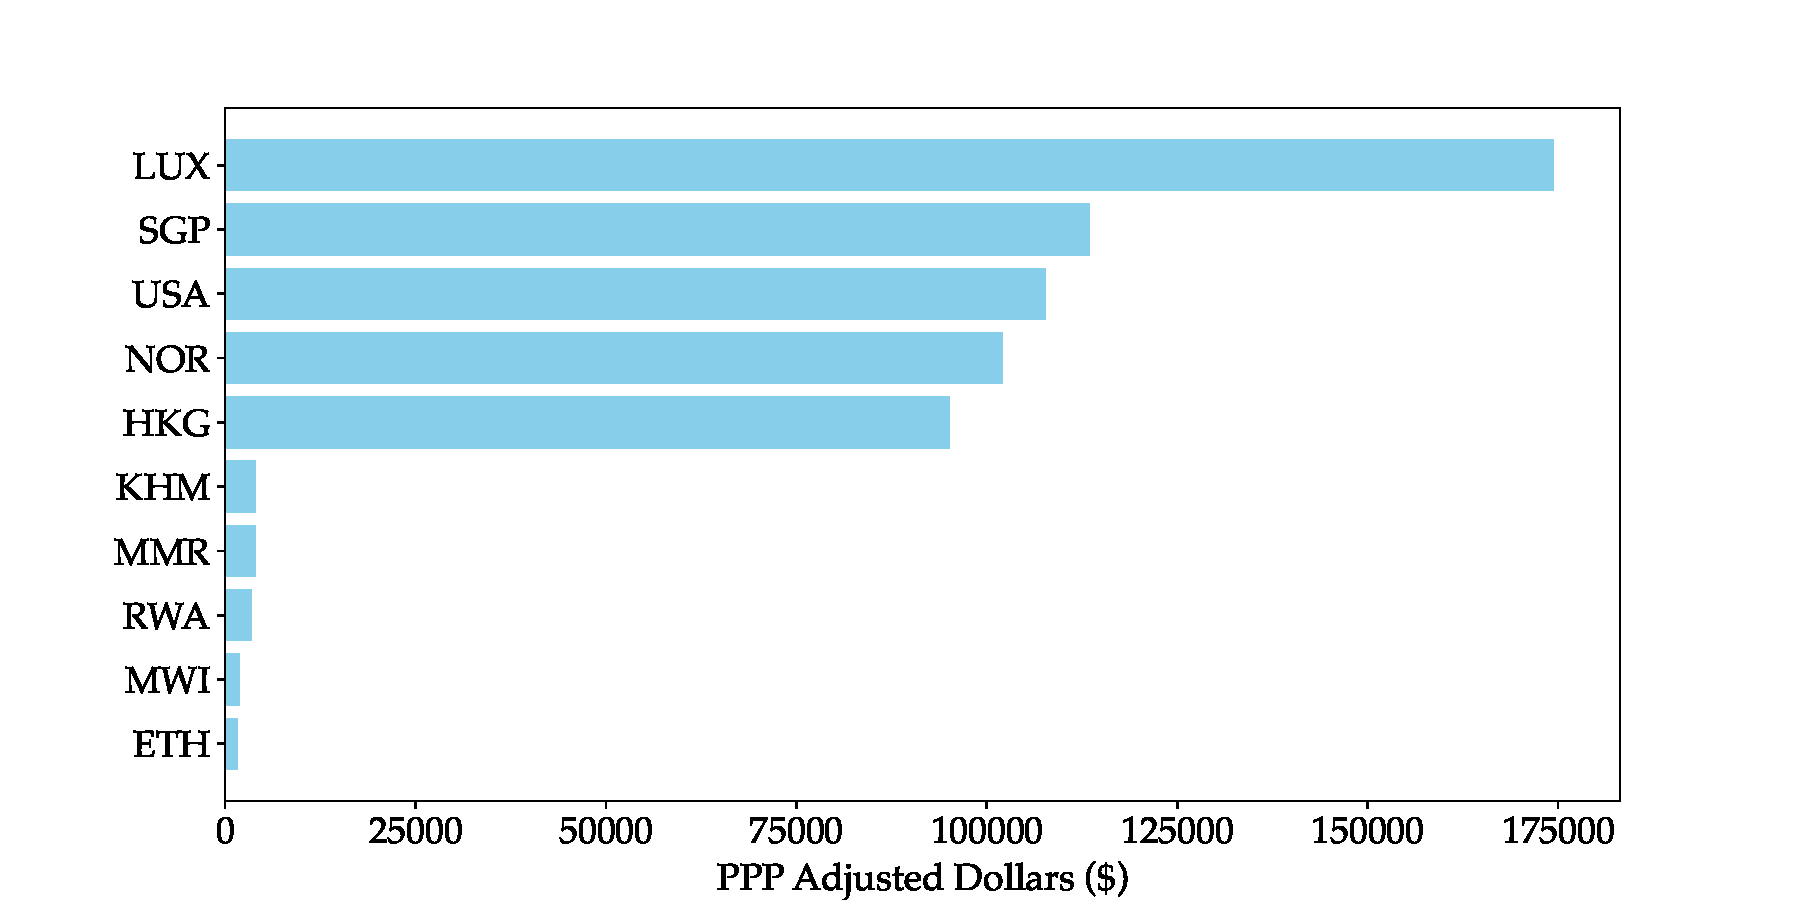
\includegraphics[width = \linewidth]{horizontal_chart.pdf}

\captionof{figure}{Value Added per Worker, Top 5 and Bottom 5 Countries}
\end{center}

Poorer countries tend to also have a large \emph{nominal} APG, within the
sectors of its own economy, yet focus a much larger share of their workforce
on agriculture, leading to the question of what the aggregate impact of these sectoral
allocations and productivity gaps are.

\begin{center}
    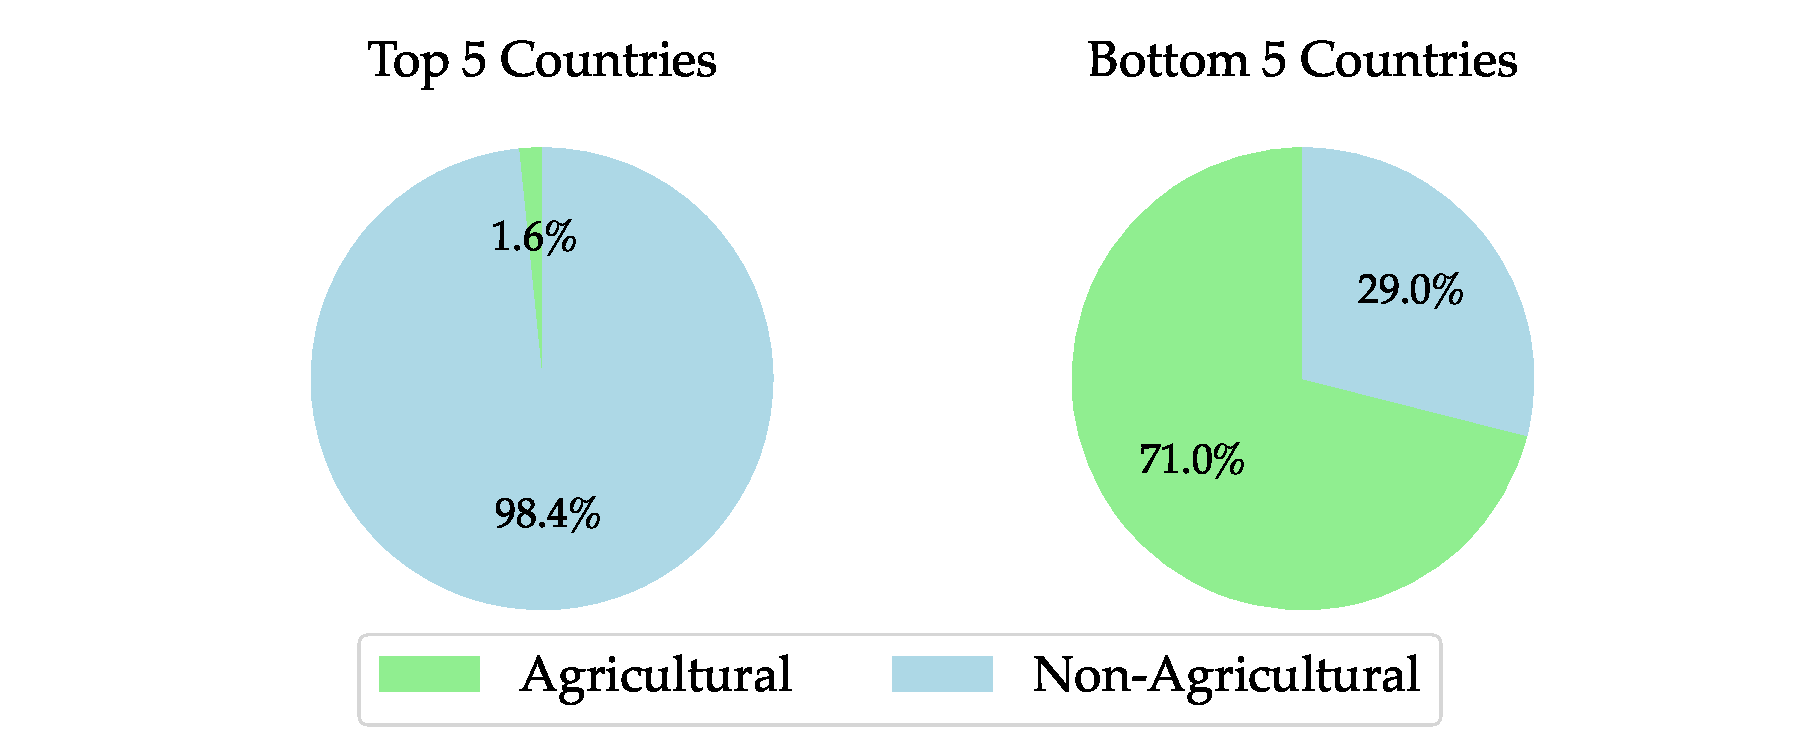
\includegraphics[width = \linewidth]{employment_share_top5_bottom5.pdf}
    \captionof{figure}{Average Employment Shares of Top 5 and Bottom 5 Countries, Ranked by Value Added per Worker}
\end{center}


% When there are two boxes, some whitespace may need to be added if the one on the right has more content
}


----------------------------------------------------------------------------------------
	RESOURCES
----------------------------------------------------------------------------------------

\headerbox{Resources}{name=resources,column=2, above = bottom, aligned = acknowledgements}{ 



\begin{itemize}[noitemsep, topsep=0pt, left=10pt]
    \item Email: \texttt{nikhil.raman@mail.mcgill.ca}
    \item GitHub: \texttt{github.com/nraman-gz}
\end{itemize}

All files for reproducing the data, figures and poster are available on GitHub.
}


%----------------------------------------------------------------------------------------
%	OBJECTIVES
%----------------------------------------------------------------------------------------

% \headerbox{Objectives}{name=introduction,column=1,row=0,bottomaligned=objectives}{

% Aliquam non lacus dolor, \textit{a aliquam quam}. Cum sociis natoque penatibus et magnis dis parturient montes, nascetur ridiculus mus. Nulla in nibh mauris. Donec vel ligula nisi, a lacinia arcu. Sed mi dui, malesuada vel consectetur et, egestas porta nisi. Sed eleifend pharetra dolor, et dapibus est vulputate eu. \textbf{Integer faucibus elementum felis vitae fringilla.} In hac habitasse platea dictumst. Duis tristique rutrum nisl, nec vulputate elit porta ut. Donec sodales sollicitudin turpis sed convallis. Etiam mauris ligula, blandit adipiscing condimentum eu, dapibus pellentesque risus.
% }

%----------------------------------------------------------------------------------------
%	RESULTS 1
%----------------------------------------------------------------------------------------

\headerbox{Cross-Sectional Data}{name=crosssection,column=1,span=2,row=0}{

\begin{multicols}{2}
\begin{minipage}{\linewidth}
    \begin{center}
        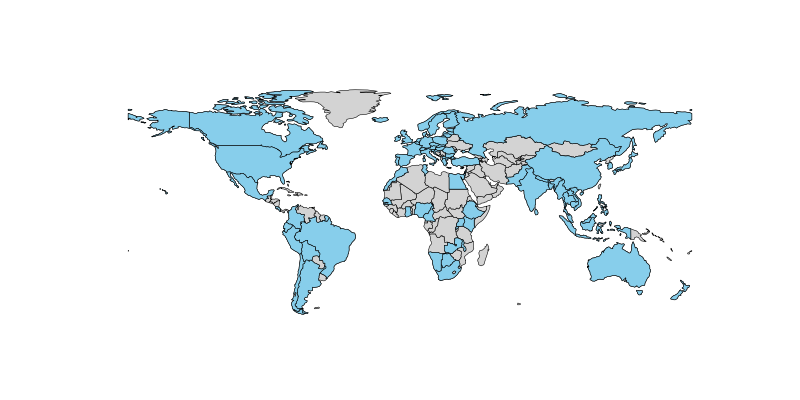
\includegraphics[scale = 0.4]{highlighted_world_map.png}
        \captionof{figure}{Countries Included in the Dataset}
    \end{center}
    
    In Figure 4, we summarize the real APG, i.e. the productivity differences across
    countries. In particular, the richest 5 countries are 60 times more
    productive in agriculture, but only 13 times more in other sectors. 

    \begin{center}
        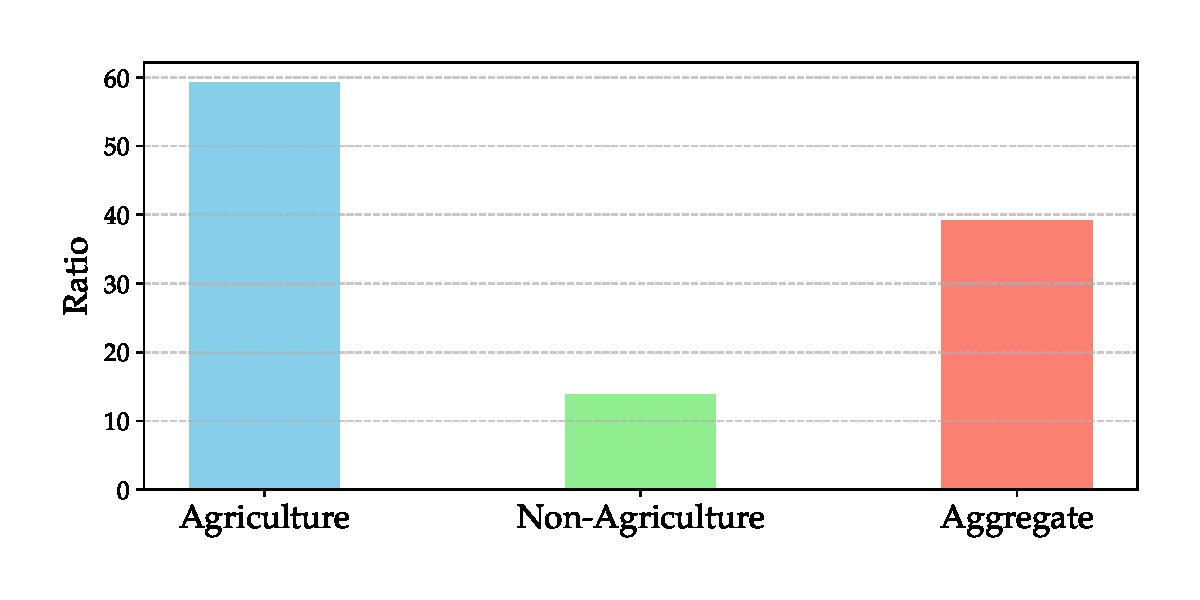
\includegraphics[width=0.8\linewidth]{sectoral_prod_top5_bottom5.pdf}
        \captionof{figure}{Ratio of Average Real Sectoral Productivity of Top 5 and Bottom 5 Countries, Ranked by Value Added per Worker}
    \end{center}

\end{minipage}

\columnbreak

We combined data from the GGDC PLD \cite{inklaar2024tradability} and
    UNSD AMA to get a sectoral
    breakdown of value added across countries in nominal terms. However, to make
    cross-country comparisons, 
    expressed in a common currency (PPP index) to make comparisons, but we only had data for the
    aggregate and agriculture sectors, so our work lay in generating a PPP index for
    non-agriculture. 


\begin{center}
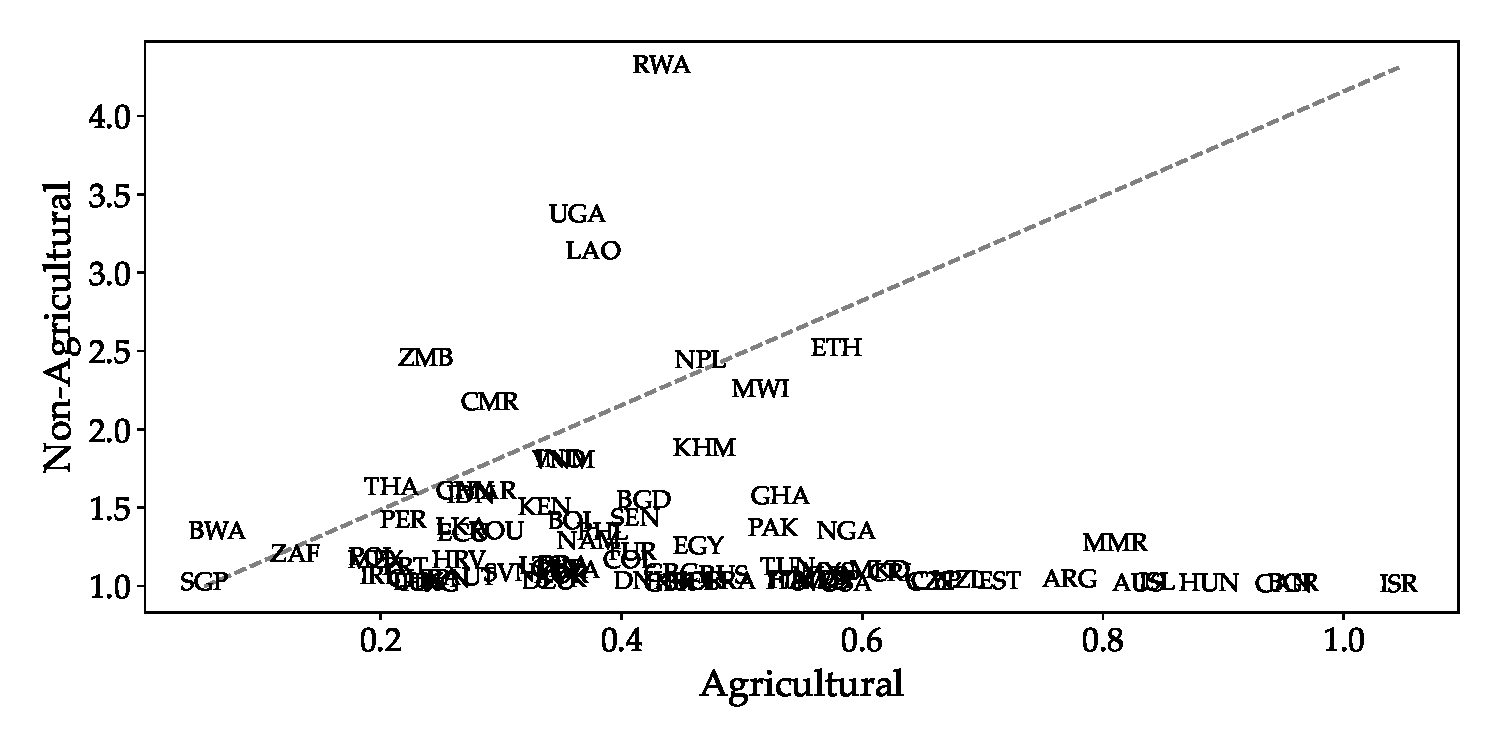
\includegraphics[width=\linewidth]{nominalAPG.pdf}
\captionof{figure}{Nominal Value Added Shares in Agriculture and Non-Agriculture}
\end{center}
Figure 5 shows the nominal APG of the data by comparing non-agricultural
productivity to its agricultural counterpart within each country. 
\end{multicols}
}


%----------------------------------------------------------------------------------------
%	RESULTS 2
%----------------------------------------------------------------------------------------

\headerbox{Time-Series Data}{name=timeseries,column=1,span=2, below=crosssection, above=acknowledgements}{


\begin{minipage}[t]{0.35\textwidth}
We took our index from the cross sectional case and extended it to all the years
    in our database, obtaining PPP adjusted sectoral value added from 1970-2023.
    Many countries showed an increasing APG and lower agriculture sectoral employment
    shares over time, following the trend of their development. 
\end{minipage}%
\hfill
\begin{minipage}[t]{0.6\textwidth}
    \begin{center}
    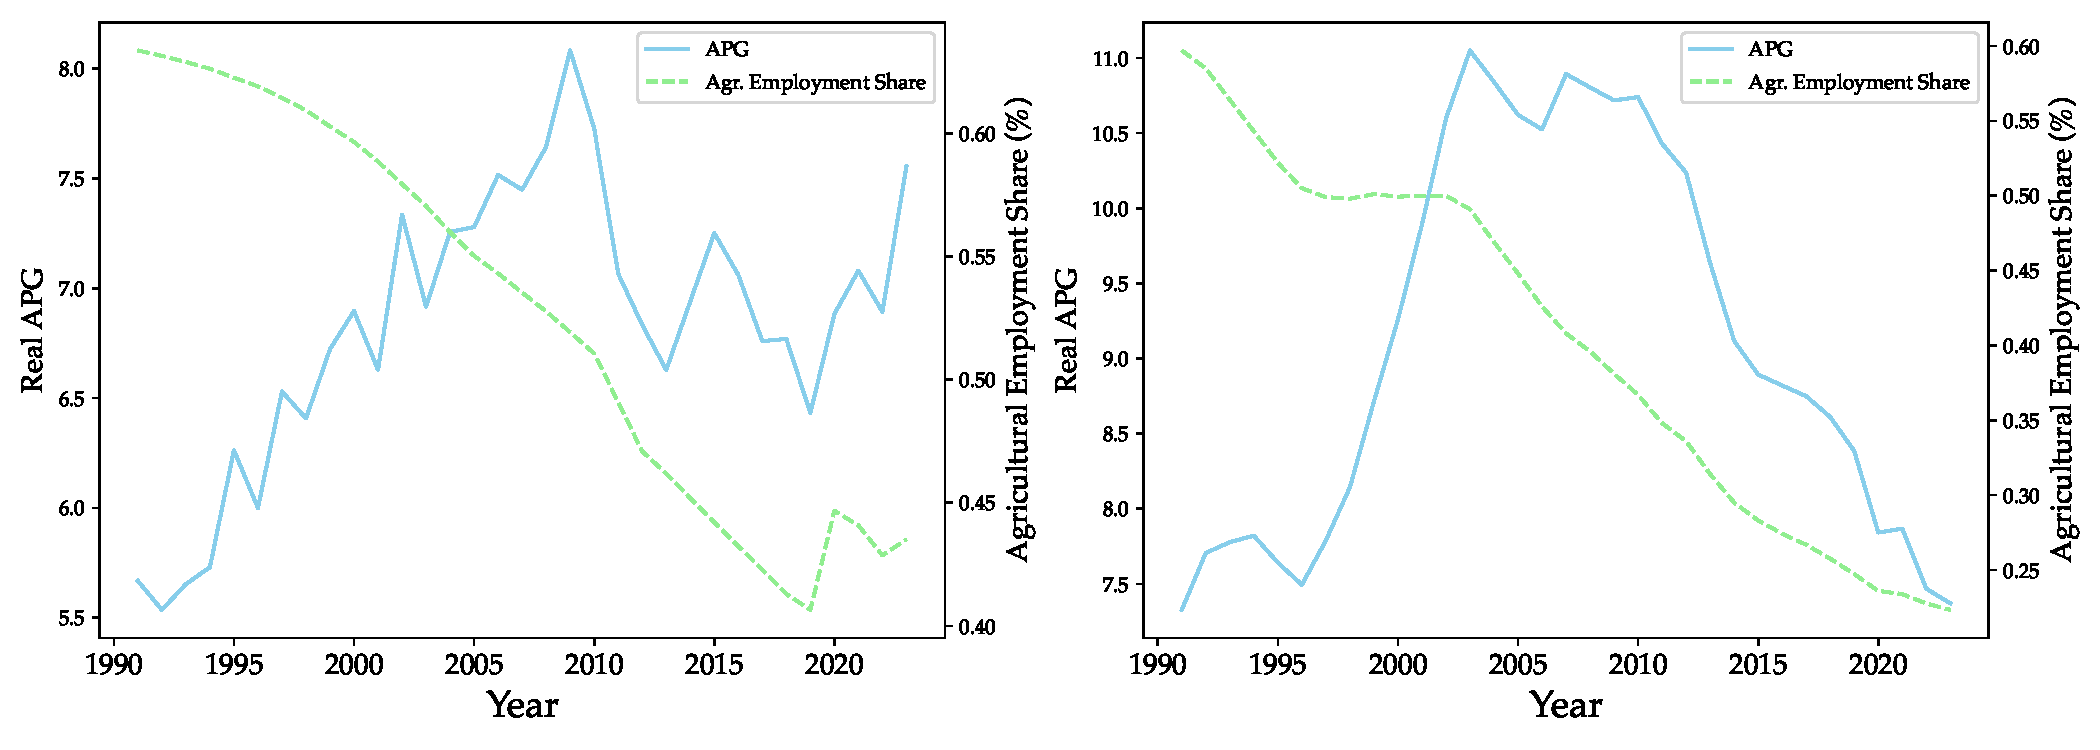
\includegraphics[scale = 0.272]{time_series.pdf}
    \captionof{figure}{Real APG and Agricultural Employment Share in India (left) and China (right), 1990-2023}
    \end{center}
\end{minipage}

% \begin{multicols}{2}

% We took our index from the cross sectional case and extended it to all the years
% in our database. Although we have sectoral value added numbers from 1970-2023, we only had
% employment numbers from 1991. Figure 6 is one example of an inverse trend in APGs and
% Employment shares in a country as it gets richer. Other countries like Brazil
% showed APG and employment shares comoving.

% \columnbreak

% \begin{center}
%     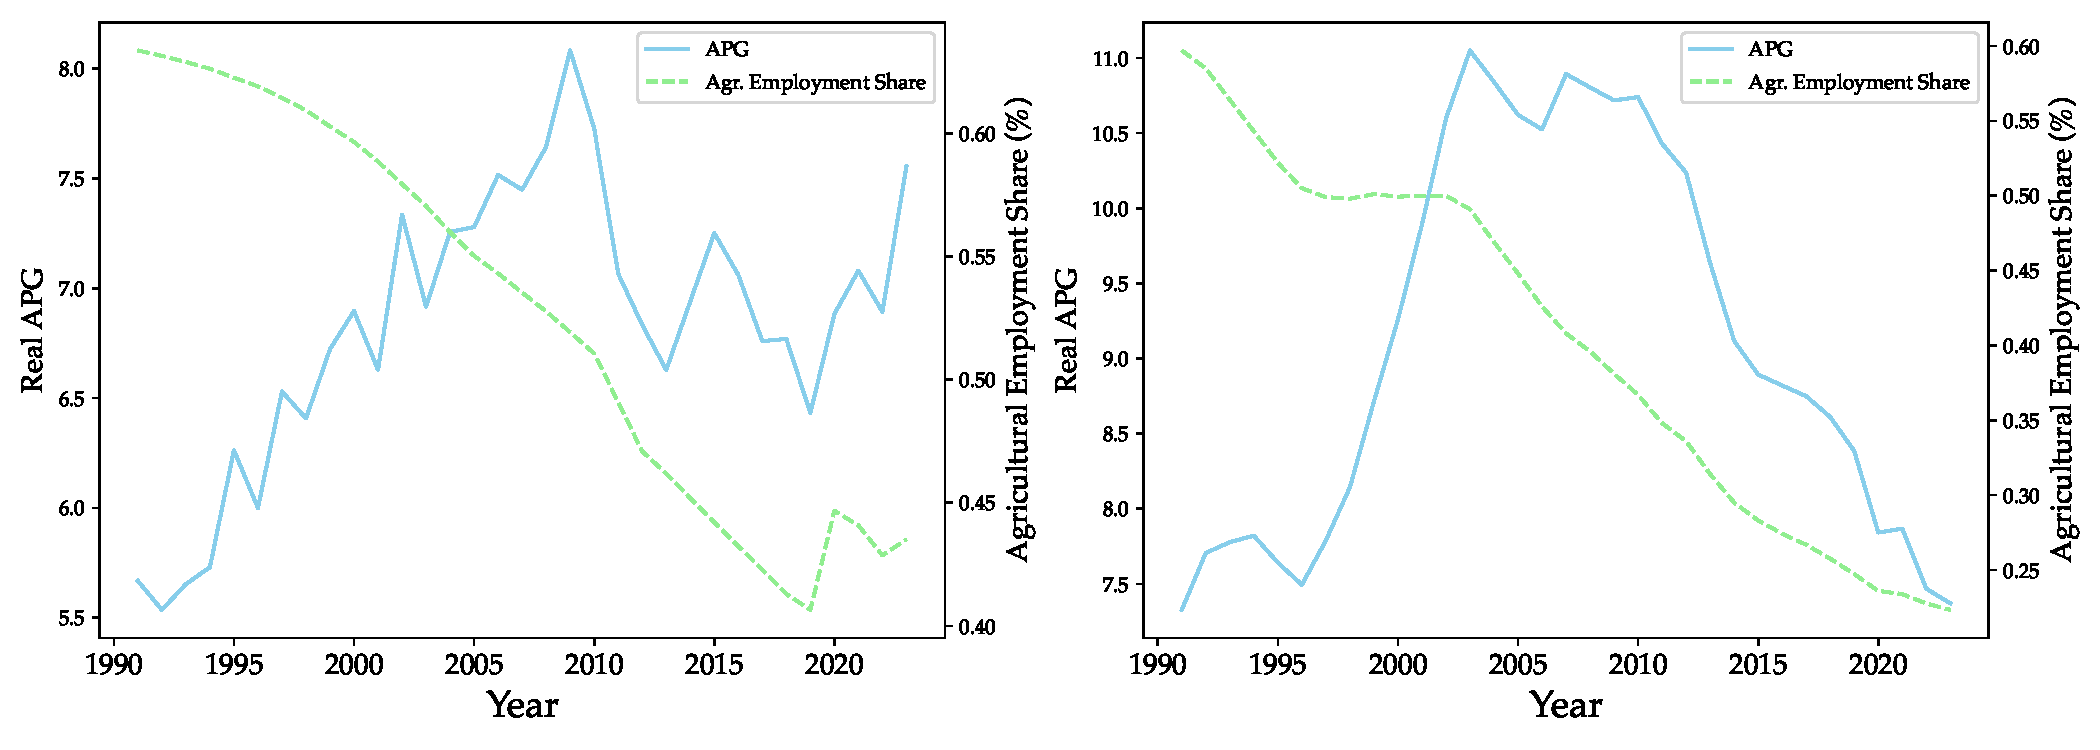
\includegraphics[width = 0.8\linewidth]{time_series.pdf}
%     \captionof{figure}{Real APG and Agricultural Employment Share in China, 1990-2023}
% \end{center}

% \end{multicols}

}




%----------------------------------------------------------------------------------------
%	REFERENCES
%----------------------------------------------------------------------------------------

\headerbox{References}{name=references,column=3, row = 4,span = 1,above=bottom}{

\renewcommand{\section}[2]{\vskip 0.05em} % Get rid of the default "References" section title
% Insert publications even if they are not cited in the poster
\scriptsize{ % Reduce the font size in this block
\begin{thebibliography}{1}
\setlength{\itemsep}{-2pt}
\bibitem{restuccia2008agriculture}
Diego Restuccia, Dennis~Tao Yang, and Xiaodong Zhu.
\newblock Agriculture and aggregate productivity: A quantitative cross-country analysis.
\newblock {\em Journal of monetary economics}, 55(2):234--250, 2008.

\bibitem{inklaar2024tradability}
Robert Inklaar, Ryan Marapin, and Kaira Gr{\"a}ler.
\newblock Tradability and sectoral productivity differences across countries.
\newblock {\em IMF Economic Review}, pages 1--53, 2024.

\bibitem{feenstra2015next}
Robert~C Feenstra, Robert Inklaar, and Marcel~P Timmer.
\newblock The next generation of the penn world table.
\newblock {\em American economic review}, 105(10):3150--3182, 2015.

\end{thebibliography}

}}


----------------------------------------------------------------------------------------
	APPENDIX
----------------------------------------------------------------------------------------

\headerbox{Appendix: Math}{name=appendix,column=3,above = references}{ % This block is as tall as the references block
A Purchasing Power Parity (PPP) adjustment is required to make any
comparisons of goods across economies, but what actually is it? Exchange simply rates
express one country's currency in another's, but that doesn't ensure
the values are equal \footnote{e.g., \$1 USD = \$1.38 CAD, but \$1 USD buys 1 apple in
the US whereas \$1.38 CAD buys 2 in Canada}.
Following the method of PWT \cite{feenstra2015next}, we first take
the ratio of nominal and real value added to get the nominal price: 
{\condensemath
    \[p_i^x = \frac{\mathit{VA}_i^{x, nom}}{\mathit{VA}_i^{x, real}}\]
}
where \(i\) is a sector, and \(x \in C\) is a country.
We use a composite index to convert prices into a PPP index for our
\(\mathit{VA}\)s. 
We then use the Geary-Khamis Method to make the PPP sectoral \(\mathit{VA}\)s
additive. It obtains a vector \(\mathit{PPP}_{all}\) by first calculating a reference
price
{\condensemath
\[\pi_i = \frac{\sum_{j \in C}\mathit{VA}_i^{j, nom}/\mathit{PPP}_{all}^j}{\sum_{j \in
C}\mathit{VA}_i^{j, nom}/\mathit{PPP}_{i}^j}\]}
and minimizing the difference between it and the observed price:
{\condensemath
    \[\mathit{PPP}_{all}^{x, obs} = \frac{VA^{x,nom}_i}{\pi_i \cdot \mathit{VA}_i^{j,
nom}/\mathit{PPP}_{i}^j} \text{ for \(x \in C\)}\]}
Using this PPP, we can use nominal prices for any year
and multiply to extend our PPPs to all years in the data
{\condensemath\[\mathit{PPP}_{i,t}^x = \mathit{PPP}_{all, BY}^x \cdot \frac{p_{i,t}^x}{p_{i, BY}^x}\]}
where \(BY\) is the base year.
}

%----------------------------------------------------------------------------------------
%	ACKNOWLEDGEMENTS
%----------------------------------------------------------------------------------------

% \headerbox{Acknowledgements}{name=contact,column=3,aligned=references,above=bottom}{ % This block is as tall as the references block

% I would like to thank Professor Francisco Alvarez-Cuadrado for including me in
% this project and for his guidance throughout the process, as well as
% Ph.D. candidate Shu Chen for his ideas and work. I also thank the Mark W. Gallop
% Foundation for funding this research. 
% }

%----------------------------------------------------------------------------------------
%	CONCLUSION
%----------------------------------------------------------------------------------------

% \headerbox{Conclusion}{name=conclusion,column=2,span=2,row=0,below=results,above=references}{

% \begin{multicols}{2}

% \tikzstyle{decision} = [diamond, draw, fill=blue!20, text width=4.5em, text badly centered, node distance=2cm, inner sep=0pt]
% \tikzstyle{block} = [rectangle, draw, fill=blue!20, text width=5em, text centered, rounded corners, minimum height=4em]
% \tikzstyle{line} = [draw, -latex']
% \tikzstyle{cloud} = [draw, ellipse, fill=red!20, node distance=3cm, minimum height=2em]

% \begin{tikzpicture}[node distance = 2cm, auto]
% \node [block] (init) {Initialize Model};
% \node [cloud, left of=init] (Start) {Start};
% \node [cloud, right of=init] (Start2) {Start Two};
% \node [block, below of=init] (init2) {Initialize Two};
% \node [decision, below of=init2] (End) {End};
% \path [line] (init) -- (init2);
% \path [line] (init2) -- (End);
% \path [line, dashed] (Start) -- (init);
% \path [line, dashed] (Start2) -- (init);
% \path [line, dashed] (Start2) |- (init2);
% \end{tikzpicture}

% %------------------------------------------------

% \begin{itemize}\compresslist
% \item Pellentesque eget orci eros. Fusce ultricies, tellus et pellentesque fringilla, ante massa luctus libero, quis tristique purus urna nec nibh. Phasellus fermentum rutrum elementum. Nam quis justo lectus.
% \item Vestibulum sem ante, hendrerit a gravida ac, blandit quis magna.
% \item Donec sem metus, facilisis at condimentum eget, vehicula ut massa. Morbi consequat, diam sed convallis tincidunt, arcu nunc.
% \item Nunc at convallis urna. isus ante. Pellentesque condimentum dui. Etiam sagittis purus non tellus tempor volutpat. Donec et dui non massa tristique adipiscing.
% \end{itemize}

% \end{multicols}
% }

%----------------------------------------------------------------------------------------
%	MATERIALS AND METHODS
%----------------------------------------------------------------------------------------

% \headerbox{Materials \& Methods}{name=method,column=0,below=objectives,bottomaligned=conclusion}{ % This block's bottom aligns with the bottom of the conclusion block

% The following materials were required to complete the research:

% \begin{itemize}\compresslist
% \item Curabitur pellentesque dignissim
% \item Eu facilisis est tempus quis
% \item Duis porta consequat lorem
% \item Eu facilisis est tempus quis
% \end{itemize}

% The following equations were used for statistical analysis:

% \begin{equation}
% \cos^3 \theta =\frac{1}{4}\cos\theta+\frac{3}{4}\cos 3\theta
% \label{eq:refname}
% \end{equation}\

% \begin{equation}
% E = mc^{2}
% \label{eqn:Einstein}
% \end{equation}

% Phasellus imperdiet, tortor vitae congue bibendum, felis enim sagittis lorem, et volutpat ante orci sagittis mi. Morbi rutrum laoreet semper. Morbi accumsan enim nec tortor consectetur non commodo nisi sollicitudin. Proin sollicitudin. Pellentesque eget orci eros. Fusce ultricies, tellus et pellentesque fringilla, ante massa luctus libero, quis tristique purus urna nec nibh.
% }

%----------------------------------------------------------------------------------------
%	RESULTS 2
%----------------------------------------------------------------------------------------

% \headerbox{Results 2}{name=results2,column=1,below=objectives,bottomaligned=conclusion}{ % This block's bottom aligns with the bottom of the conclusion block

% Donec faucibus purus at tortor egestas eu fermentum dolor facilisis. Maecenas tempor dui eu neque fringilla rutrum. Mauris \emph{lobortis} nisl accumsan.

% \begin{center}
% \begin{tabular}{l l l}
% \toprule
% \textbf{Treatments} & \textbf{Response 1} & \textbf{Response 2}\\
% \midrule
% Treatment 1 & 0.0003262 & 0.562 \\
% Treatment 2 & 0.0015681 & 0.910 \\
% Treatment 3 & 0.0009271 & 0.296 \\
% \bottomrule
% \end{tabular}
% \captionof{table}{Table caption}
% \end{center}

% Nulla ut porttitor enim. Suspendisse venenatis dui eget eros gravida tempor. Mauris feugiat elit et augue placerat ultrices. Morbi accumsan enim nec tortor consectetur non commodo.

% \begin{center}
% \begin{tabular}{l l l}
% \toprule
% \textbf{Treatments} & \textbf{Response 1} & \textbf{Response 2}\\
% \midrule
% Treatment 1 & 0.0003262 & 0.562 \\
% Treatment 2 & 0.0015681 & 0.910 \\
% Treatment 3 & 0.0009271 & 0.296 \\
% \bottomrule
% \end{tabular}
% \captionof{table}{Table caption}
% \end{center}
% }

%----------------------------------------------------------------------------------------

\end{poster}

\end{document}